\documentclass[fleqn]{article}

\usepackage{mydefs}
\usepackage{notes}
\usepackage{url}
\usepackage{graphicx}


\begin{document}
\lecture{Computer Vision}{HW03: White balance}{CS 670, Fall 2016}

% IF YOU ARE USING THIS .TEX FILE AS A TEMPLATE, PLEASE REPLACE
% "CS 726, Fall 2011" WITH YOUR NAME AND UID.

Hand in via moodle at: \url{https://moodle.umass.edu/course/view.php?id=33024}.
Remember that only PDF submissions are accepted.  We encourage using
\LaTeX\ to produce your writeups.  See \verb+hw00.tex+ for an example
of how to do so.  You can make a \verb+.pdf+ out of the \verb+.tex+ by
running ``\verb+pdflatex hw00.tex+''.

\vspace{0.2in}

Our eyes are very good at removing the effect of illumination to judge the true color of an object. A simple way of modeling the effect of a light is to assume that the reflected color $I = (i_r,i_g,i_b)$ arises due to a light $L= (l_r,l_g,l_b)$ interacting with paint $C = (c_r,c_g,c_b)$ satisfying  
	$L \times C = I$, i.e. at each pixel we have
	$(l_r \times c_r,l_g \times c_g ,\l_b \times c_b) = (i_r,i_g,i_b)$.

Computing $L$ and $C$ given $I$ is ill-posed. For example, a red pixel in an image $I=(255,0,0)$ might be due to a white light $L=(1,1,1)$ on a red object $C=(255,0,0)$, or red light $L=(1,0,0)$ on a white object $C=(255,255,255)$. Thus, in order to solve this problem certain priors are needed. One such prior is the ``gray world" assumption that states the average color of the image under white light is gray (Recall that any color $(r,g,b)$ where $r=g=b$ is gray). 

\begin{itemize}
\item Assume that the average color of an image under white light $L=(1,1,1)$ is $(128,128,128)$. Under this assumption, show that given an image the color of the light can be computed as 
	$ L = \left(\frac{r_{ave}}{128}, \frac{g_{ave}}{128}, \frac{b_{ave}}{128}\right)$, where, $r_{ave}, g_{ave}, b_{ave}$ are the average red, green, and blue values of the image. 

\item Thus, you can obtain the true color of a pixel as: $
	c_r = i_r \times \frac{128}{r_{ave}}; 
	c_g = i_g \times \frac{128}{g_{ave}}; 
	c_b = i_b \times \frac{128}{b_{ave}}; $\\
Implement a function in Matlab that takes an image $I$ and returns the light $L$ and color image $C$ using the above calculations. Run your code on the included image \texttt{wb\_sardmen-incorrect.jpg} (Figure~\ref{fig:color}).  Write down the value of $L$ below and include a picture of the color corrected image (using \texttt{imagesc(C); axis image off;}) in your solution.\\ \\
\textbf{Light}~~ $l_r$: \underline{\hspace{2cm}}, $l_g$: \underline{\hspace{3cm}}, $l_b$:\underline{\hspace{3cm}}
\end{itemize}

\begin{figure}[h]
\centering
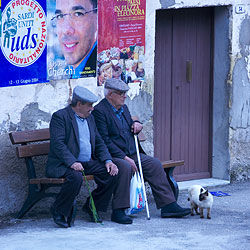
\includegraphics[scale=0.75]{wb_sardmen-incorrect.jpg}
\caption{\label{fig:color} Image with a color cast}
\end{figure}
Image source: \url{http://www.cambridgeincolour.com/tutorials/white-balance.htm}

\end{document}
